\section{Results}
\label{sec:results}

In the main text, we focus on the first batch. Additional results for Batch 2, both batches combined, and the intensive-margin specifications are presented in Appendix~\ref{app:results_appendix}.

\subsection{First Stage: Batch 1}

\begin{table}[!htbp]
\centering
\caption{First Stage Extensive - All Transforms (Batch 1)}
\begin{tabular}{lcccccccc}
\hline
 & \multicolumn{2}{c}{IHS (arcsinh)} & \multicolumn{2}{c}{log(y+1)} & \multicolumn{2}{c}{Dummy (y>0)} & \multicolumn{2}{c}{Chen-Roth} \\
 & Ads & SMI & Ads & SMI & Ads & SMI & Ads & SMI \\
\hline
Total Treated & 0.000 & 0.002*** & 0.000 & 0.002*** & 0.000 & 0.001*** & 0.000 & 0.002*** \\
 & (0.000) & (0.001) & (0.000) & (0.001) & (0.000) & (0.000) & (0.000) & (0.001) \\
Pure ctrl mean & 0.0000 & 0.0002 & 0.0000 & 0.0001 & 0.0000 & 0.0001 & -1.0000 & -0.9998 \\
\hline
\multicolumn{9}{l}{\parbox[t]{15.5cm}{\textit{Notes:} Standard errors are permutation-based. Significance stars: * p<0.10, ** p<0.05, *** p<0.01.}} \\
\end{tabular}
\end{table}


\subsection{Null Effects on Extensive Outcomes: Batch 1}

\begin{figure}[!htbp]
    \centering
    \caption{Extensive Outcomes: Baseline and Endline Effects, Batch 1}
    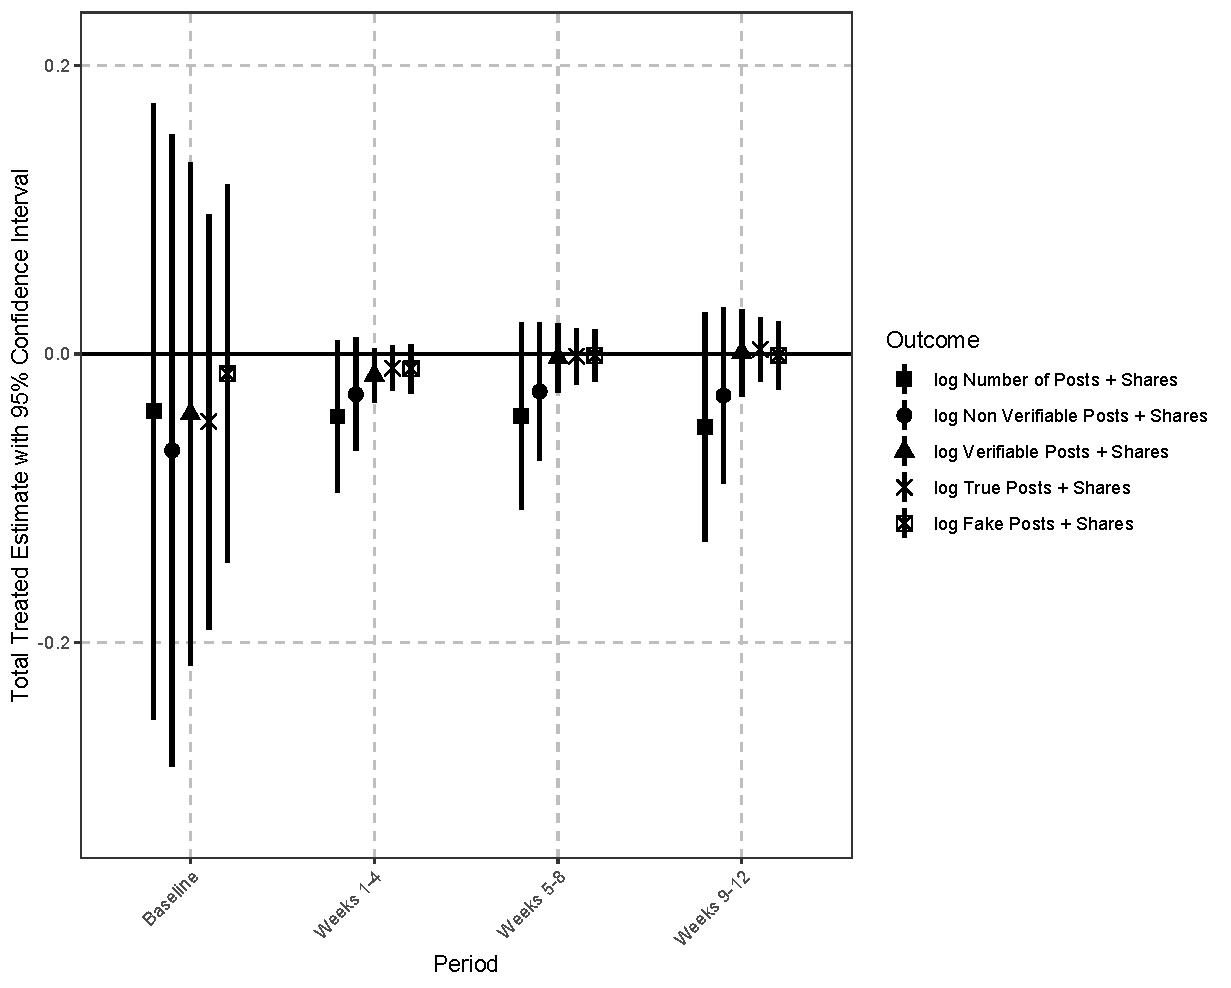
\includegraphics[width=\textwidth]{../results/replots/extensive_linear_90p_p5_with_baseline/log_extensive_verifiability_fes_normal_p90_p5_b1_500perm_with_baseline.pdf}
    \label{fig:extensive_b1_baseline_endline}
    \floatfoot{\textit{Notes:} The figure reports the estimated effect of treatment for the Batch 1 sample, combining the baseline specification with the endline specifications for Weeks 1--4, Weeks 5--8, and Weeks 9--12. Whiskers denote permutation-based 95\% confidence intervals.}
\end{figure}

\subsection{Robustness: Strong Followers Only, Batch 1}

\begin{figure}[!htbp]
    \centering
    \caption{Extensive Outcomes: Baseline and Endline Effects, Strong-Follower Sample, Batch 1}
    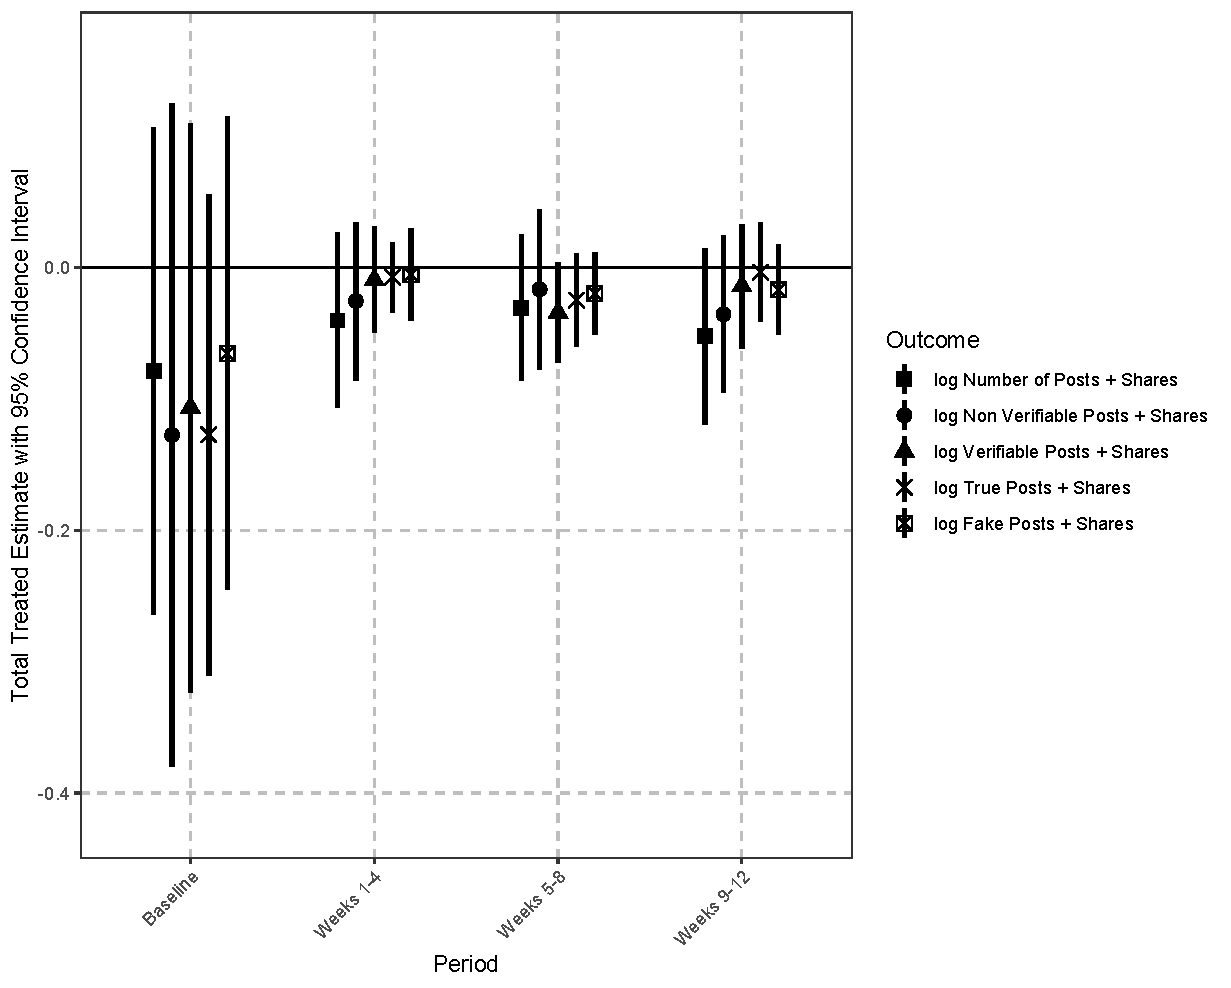
\includegraphics[width=\textwidth]{../results/replots/extensive_linear_90p_p5_strong_with_baseline/log_extensive_verifiability_fes_normal_p90_p5_strong_b1_500perm_with_baseline.pdf}
    \label{fig:extensive_strong_b1_baseline_endline}
    \floatfoot{\textit{Notes:} The figure reports the estimated effect of treatment for the Batch 1 sample restricted to followers with at least one strong treated connection. Whiskers denote permutation-based 95\% confidence intervals.}
\end{figure}
